% !TEX TS-program = pdflatex
% !TEX encoding = UTF-8 Unicode

% This is a simple template for a LaTeX document using the "article" class.
% See "book", "report", "letter" for other types of document.

\documentclass[11pt]{article} % use larger type; default would be 10pt


\usepackage[utf8]{inputenc} % set input encoding (not needed with XeLaTeX)

%%% Examples of Article customizations
% These packages are optional, depending whether you want the features they provide.
% See the LaTeX Companion or other references for full information.

%%% PAGE DIMENSIONS
\usepackage{geometry} % to change the page dimensions
\geometry{a4paper} % or letterpaper (US) or a5paper or....
% \geometry{margin=2in} % for example, change the margins to 2 inches all round
% \geometry{landscape} % set up the page for landscape
%   read geometry.pdf for detailed page layout information

\usepackage{graphicx} % support the \includegraphics command and options

% \usepackage[parfill]{parskip} % Activate to begin paragraphs with an empty line rather than an indent

%%% PACKAGES
\usepackage{booktabs} % for much better looking tables
\usepackage{array} % for better arrays (eg matrices) in maths
\usepackage{paralist} % very flexible & customisable lists (eg. enumerate/itemize, etc.)
\usepackage{verbatim} % adds environment for commenting out blocks of text & for better verbatim
 % make it possible to include more than one captioned figure/table in a single float
% These packages are all incorporated in the memoir class to one degree or another...

\usepackage[export]{adjustbox}
\usepackage{graphicx}
\usepackage{amssymb}
\usepackage{hyperref}
\hypersetup{
    colorlinks=true,
    linkcolor=blue,
    filecolor=magenta,      
    urlcolor=cyan,
}
\usepackage{relsize}
\usepackage[utf8]{inputenc}
\usepackage[LGR]{fontenc}
\usepackage[T1]{fontenc}
\usepackage[greek,english]{babel}
\usepackage{alphabeta}
\usepackage{amsmath}
\usepackage{physics}
\usepackage{amsfonts}
\usepackage{nccmath}
\usepackage[overload]{empheq}
\usepackage{float}
\usepackage{caption}
\usepackage{subcaption}
\restylefloat{table}
\usepackage{afterpage}
\usepackage[nottoc,notlot,notlof]{tocbibind}
\addto\captionsenglish{\renewcommand{\tablename}{Πίνακας}}
\addto\captionsenglish{\renewcommand{\figurename}{Εικόνα}}


\begin{document}

\begin{titlepage}
    \begin{center}
        \vspace*{1cm}
	
\includegraphics[width=0.2\textwidth]{plots/ntua_logo}\\    
	\vspace*{1cm}
        \Huge
        \textbf{Αναγνώριση Προτύπων}
            
        \vspace{0.5cm}
        \LARGE
        Εργασία 1η
            
        \vspace{1.5cm}
        
        \textbf{Μιχάλης Στεφανής }\\
	  (Α.Μ. 03400156)    \\
        \textbf{Βασίλης Μηναδάκης }\\
	  (Α.Μ. 03400143)
            
        \vfill
                        
        \vspace{0.8cm}
            
        
            
        \Large
        Σχολή Ηλεκτρολόγων Μηχανικών και Μηχανικών Υπολογιστών\\
        Εθνικό Μετσόβιο Πολυτεχνείο\\
        Αθήνα\\
        24/10/2021
            
    \end{center}
\end{titlepage}

\underline{\textbf{Βήμα 1}}\\

Για την επίλυση όλων των ερωτημάτων έγινε η χρήση των βιβλιοθηών numpy, scikit-learn και matplotlib της python.\\
Το πρώτο στάδιο αφορά την εισαγωγή των train και test δεδομένων από μορφή αρχείου κειμένου (.txt) στον κώδικα της python. Αυτό επιτυγχάνεται με τη χρήση της συνάρτησης $np.genfromtxt()$. Έπειτα, ακολουθώντας τις οδηγίες της εκφώνησης δημιουργήθηκαν ρα εξής arrays δεδομένων:

\begin{table}[h]
\begin{center}
\begin{tabular}{c c }
\hline\hline
Ονομασία & Διαστάσεις \\
\hline
train\_features & 7291x256\\ 
train\_labels     & 7291      \\  
test\_features  & 2007x256\\
test\_labels      & 2007\\
\hline 
\end{tabular}
\caption{Διαστάσεις των training και test dataset.}
\end{center}
\end{table}

\underline{\textbf{Βήμα 2}}\\

Στο \textbf{2ο βήμα} σχεδιάστηκε το υπ'αριθμόν 131 ψηφίο των train δεδομένων χρησιμοποιώντας συναρτήσεις της βιβλιοθήκης matplotlib και συγκεκριμένα της $plt.imshow()$ και $plt.show()$. Η πρώτη εφαρμόζεται ουσιαστικά πάνω στο 131ο στοιχείο των train\_features και η εικόνα που παράγεται είναι η κάτωθι.

\begin{figure}[H]
    \centering
    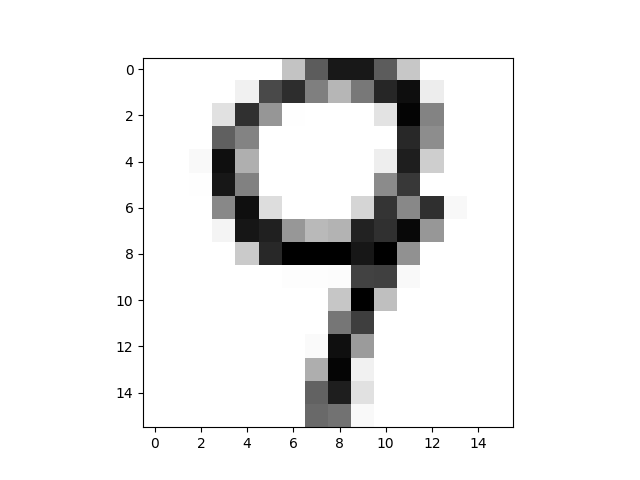
\includegraphics[width=0.7\textwidth]{plots/Step 2}
    \caption{Απεικόνιση του 131ου ψηφίου των train\_features.}
    \label{fig:step_2}
\end{figure}

\underline{\textbf{Βήμα 3}}\\

Για το \textbf{3ο βήμα} δομήθηκε η συνάρτηση $plot\_digits\_samples(X, y)$, της οποίας τα ορίσματα είναι τα training\_features και τα training\_labels αντίστοιχα. Συνοπτικά, η συγκεκριμένη συνάρτηση λειτουργεί με μία επαναληπτική διαδικασία από το 1 έως το πλήθος των στοιχείων του X (train\_features), εντός της οποίας αν το στοιχείο y(i) υπάρχει στο διάνυσμα $digits = \{0,1,...,9\}$, τότε σχεδιάζεται το αντίστοιχο ψηφίο και στη συνέχεια αφαιρείται από το διάνυσμα digits, μέχρι να μην υπάρχει κανένα στοιχείο πλέον εντός του digits. Η ενσωμάτωση των εικόνων και των 10 διαφορετικών ψηφίων σε μία εικόνα γίνεται με τη χρήση της συνάρτησης $plt.subplots()$ και παρουσιάζονται στην εικόνα \ref{fig:step_3}.

\begin{figure}[H]
    \centering
    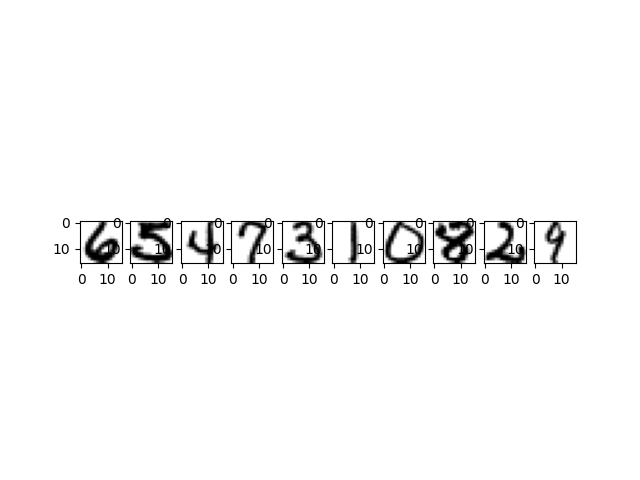
\includegraphics[width=1.1\textwidth]{plots/Step 3}
    \caption{Απεικόνιση του 131ου ψηφίου των train\_features.}
    \label{fig:step_3}
\end{figure}

\underline{\textbf{Βήμα 4}}\\

Στη συνέχεια, για την υλοποίηση του \textbf{4ου βήματος}, κατασκευάστηκε η συνάρτηση $mean\_value\_at\_pixel\_of\_digit(X, y, digit, pixel=(10, 10))$, η οποία υπολογίζει τη μέση τιμή όλων των χαρακτηριστικών ενός συγκεκριμένου pixel (συγκεκριμένα του 10ου) για το training set και δέχεται σαν input  τα train\_features, τα train\_labels και το ψηφίο που μας ενδιαφέρει (στη συγκεκριμένη περίπτωση το 0). Ο τύπος τις μέσης τιμής που χρησιμοποιήθηκε είναι η \ref{mean_value}: 

\begin{equation}
\label{mean_value}
\mu = \frac{1}{n}\bigg(\sum_{i=1}^{n}x_{i}\bigg),
\end{equation}
όπου $n$ το πλήθος των χαρακτηριστικών του pixel (10,10) για το ψηφίο 0.
\\

\underline{\textbf{Βήμα 5}}\\

Στο \textbf{βήμα 5} η λογική που ακολουθήθηκε είναι όμοια με αυτή του προηγούμενου βήματος, μόνο που σε αυτή την περίπτωση το function που δομήθηκε ($mean\_value\_at\_pixel\_of\_digit(X, y, digit, pixel=(10, 10))$) κάνει τους υπολογισμούς με βάση της διασπορά των χαρακτηριστικών, δηλαδή γίνεται χρήση της σχέσης \ref{variance}: 

\begin{equation}
\label{variance}
Var(x) = \frac{1}{n}\bigg(\sum_{i=1}^{n}(x_{i}-\mu)^{2}\bigg).
\end{equation}
Εφαρμόζοντας τις δύο παραπάνω συναρτήσεις για το 10 pixel όλων των χαρακτηριστικών του ψηφίου μηδέν προκύπτουν οι εξής τιμές για τη μέση τιμή και διασπορά του:

\begin{table}[h]
\begin{center}
\begin{tabular}{c c c}
\hline\hline
 & Μέση Τιμή & Διασπορά\\
\hline
10ο pixel του 0 & -0.5041 & 0.5245\\
\hline 
\end{tabular}
\caption{Αποτελέσματα μέσης τιμής και διασποράς του 10ου pixel όλων των στοιχείων για το ψηφίο 0.}
\end{center}
\end{table}

\underline{\textbf{Βήμα 6}}\\

Στη συνέχεια για τον υπολογισμό της μέσης τιμής και της διασποράς των χαρακτηριστικών όλων των pixel ενός οποιουδήποτε ψηφίου, δομήθηκαν οι συναρτήσεις $digit\_mean(X, y, digit)$ και $digit\_variance(X, y, digit)$. Αυτές οι δύο συναρτήσεις σε πρώτο επίπεδο υπολογίζουν τη μέση τιμή και τη διασπορά κάθε ενός pixel του επιθμητού ψηφίου και στη επιστρέφει αυτές τις τιμές σε ένα διάνυσμα. 

\underline{\textbf{Βήμα 7}}\\

Οι τελευταίες δύο συναρτήσεις χρησιμοποιούνται ως εσωτερικές της νέας συνάρτησης $plot\_digit\_mean(X, y, digit)$, η οποία χρησιμοποιείται για το σχεδιασμό ενός επιθμητού ψηφίου χρησιμοποιώντας τη μέση τιμή όλων των pixel όλων των χαρακτηριστικών του συγκεκριμένου ψηφίου. Η εικόνα που παράγεται με τη χρήση του συγκεκριμένου function για το ψηφίο 0, χρησιμοποιώντας το training set είναι η εικόνα \ref{fig:step_7}.

\begin{figure}[H]
    \centering
    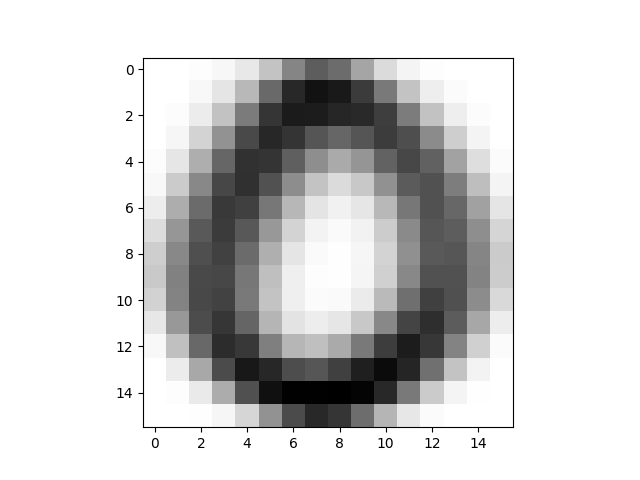
\includegraphics[width=0.7\textwidth]{plots/Step 7}
    \caption{Απεικόνιση του ψηφίου 0 με τη χρήση της μέσης τιμής των pixel όλων των χαρακτηριστικών του training set.}
    \label{fig:step_7}
\end{figure}

\underline{\textbf{Βήμα 8}}\\

Το επόμενο βήμα (\textbf{Βήμα 8}) είναι να σχεδιάσουμε ένα από τα ψηφία που επιθυμούμε χρησιμοποιώντας όχι την μέση τιμή, αλλά την διασπορά των pixel των είκονων που αντιπροσωπεύουν το επιθυμητό ψηφίο. Αυτό γίνεται με την συνάρτηση $plot\_digit\_variance$. Για παράδειγμα, για το ψηφίο $0$ παίρνουμε την εξής εικόνα:

\begin{figure}[H]
    \centering
    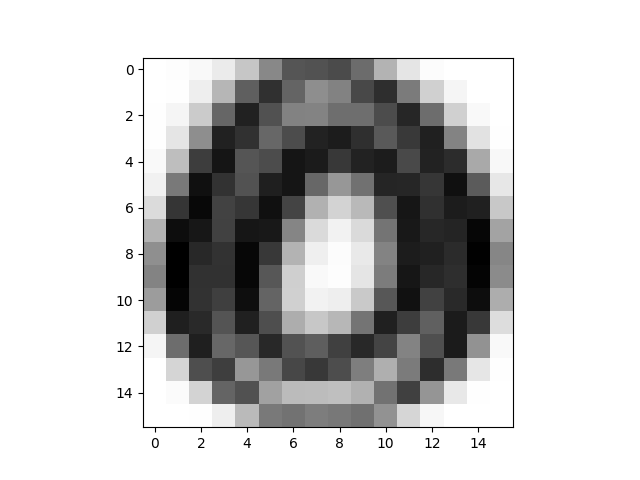
\includegraphics[width=0.7\textwidth]{plots/variance_0}
    \caption{Απεικόνιση του ψηφίου $0$ μέσω της διασποράς των pixel}
    \label{fig:var_0}
\end{figure}



Αν συγκρίνουμε την εικόνα που πήραμε από το ψηφίο 0 μέσω της μέσης τιμής με αυτήν που πήραμε μέσω τις διασποράς θα παρατηρήσουμε κάποιες σχετικά αναμενόμενες διαφορές. Η εικόνα που αντιστοιχεί στην διασπορά έχει τα πιο σκούρα της pixels αυτά που τα αντίστοιχα στην εικόνα της μέσης τιμής είναι τα λιγότερο σκούρα. Για παράδειγμα τα pixels της εικόνας της μέσης τιμής για το $0$ είναι περισσότερο σκούρα στις δύο "κορυφές" του $0$. Αντίστοιχα, τα pixels της εικόνας της διασποράς είναι λιγότερο σκούρα (περισσότερο γκρί παρά μαύρα) στις κορυφές αυτές. Αυτό είναι αναμενόμενο, καθώς η διασπορά είναι στην ουσία η απόσταση μιας μεταβλητής από την μέση τιμή της. \\

\underline{\textbf{Βήμα 9}}\\

Για το \textbf{Βήμα 9} υπολογίζουμε την μέση τιμή και την διασπορά όλων των pixel για όλα τα δεδομένα εκπαίδευσης. Αυτό μπορεί να γίνει πολύ απλά χρησιμοποιωντας list-comprehension της python και τις συναρτήσεις $digit\_mean$ και $digit\_variance$ αντίστοιχα. Παίρνουμε έτσι δύο λίστες 10 γραμμών και 256 στηλών ($mean\_X$ και $var\_X$). Κάθε γραμμή αντιστοιχεί σε ένα ψηφίο και κάθε στήλη στην μέση τιμή και την διασπορά του εκάστοτε pixel. \\

Για να σχεδιάσουμε όλα τα ψηφία χρησιμοπoιούμε τις συνάρτησεις  $plot\_digits\_by\_mean$ και $plot\_digits\_by\_variance$, οι οποίες χρησιμοποιούν 10 φορές η καθε μία τις συναρτήσεις $digit\_mean$ και $digit\_variance$ αντίστοιχα. 

\begin{figure}[H]
    \centering
    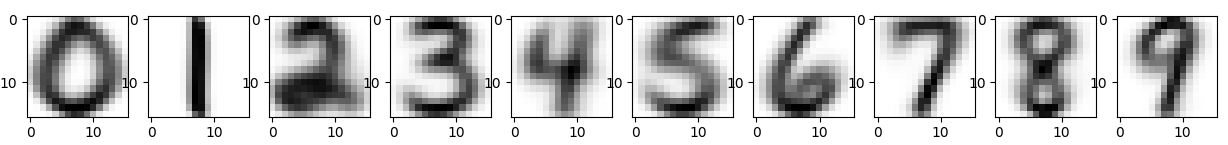
\includegraphics[width=1.1\textwidth]{plots/all_digits_mean}
    \caption{Απεικόνιση όλων των ψηφίων μέσω της μέσης τιμής των pixel}
    \label{fig:all_mean}
\end{figure}

\begin{figure}[H]
    \centering
    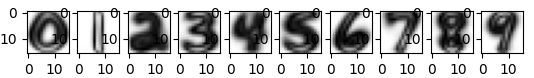
\includegraphics[width=1.1\textwidth]{plots/all_digits_variance}
    \caption{Απεικόνιση όλων των ψηφίων μέσω της διασποράς των pixel}
    \label{fig:all_var}
\end{figure}


\underline{\textbf{Βήμα 10}}\\

Από το \textbf{Βήμα 10} και μετά ξεκινούν οι δοκιμές του ταξινομητή της Ευκλείδιας απόστασης. Αυτός υλοποιείται με την βοήθεια δύο συναρτήσεων. Η συνάρτηση $euclidean\_distance$ υπολογίζει την Ευκλείδια απόσταση μεταξύ δύο διανυσμάτων (ή πινάκων) μέσω της σχέσης:

\begin{equation}
\displaystyle d(A, B) = \sqrt{(A[1] -B[1]) ^ 2 + (A[2] - B[2]) ^ 2 + \dots + (A[N] - B[N]) ^ 2}
\end{equation}

Στην συνέχεια για την ταξινόμηση των στοιχείων του test set καλούμε την συνάρτηση $euclidean\_distance\_classifier$. Η συνάρτηση αυτή παίρνει ως ορίσματα τα χαρακτηριστικά του test set (test features) καθώς και την λίστα που περιλαμβάνει τις μέσες τιμές όλων των ψηφίων του training set. Υπολογίζει για το κάθε στοιχείο του test set τις ευκλείδιες αποστάσεις του στοιχείου αυτού από τις μέσες τιμές. Επιλέγεται η μικρότερη από αυτές, η οποία ελάχιστη απόσταση είναι αντιπροσωπευτική της κλάσης στην οποία ταξινομήθηκε τελικά το στοιχείο που επιλεξαμε.\\

Ως πρώτη δοκιμή του ταξινομητή, διαλέγουμε το στοιχείο υπ'αριθμόν 101 των test δεδομένων και το δίνουμε ως είσοδο στον ταξινομητή μας. Για να έχουμε μία καλύτερη εικόνα, το στοιχείο αυτό είναι το εξής:


\begin{figure}[H]
    \centering
    \includegraphics[width=0.7\textwidth]{plots/figure_101}
    \caption{Το ψηφίο υπ'αριθμόν 101 των test δεδομένων}
    \label{fig:101}
\end{figure}

Αν τρέξουμε τον ταξινομητή μας θα διαπιστώσουμε ότι η ταξινόμηση δεν είναι σωστή. Όπως μπορούμε να διακρίνουμε στην παραπάνω εικόνα, το ψηφίο που αναπαριστά είναι το $6$. Παρόλα αυτά ο ταξινομητής δίνει την πρόβλεψη $0$. Οπότε "μπερδεύει"το παραπάνω εξάρι με μηδενικό. Αυτό δεν πρέπει να μας αποθαρρύνει αφού ένα μόνο test δεδομένο δεν αρκεί για να βγάλουμε συμπέρασμα για τον ταξινομητή μας. Εξάλλου η παραπάνω εικόνα είναι πράγματι ένα ασυνήθιστο $6$ για τα τυπικά χειρόγραφα δεδομένα.\\


\underline{\textbf{Βήμα 11}}\\

Ερχόμαστε τώρα στο \textbf{Βήμα 11}, όπου τροφοδοτούμε τον ταξινομητή μας με όλα τα test δεδομένα. Η συνάρτηση $euclidean\_distance\_classifier$ θα μας γυρίσει ένα \% ποσοστό επιτυχίας (δηλαδή τον αριθμό των δεδομένων που ταξινομήθηκαν επιτυχώς διαιρεμένο με τον συνολικό αριθμό των δεδομένων) και μία λίστα με όλες τις προβλέψεις του ταξινομητή (δηλαδή μία λίστα που θα μας λέει σε ποια κατηγορία ταξινομήθηκε το κάθε test δεδομένο). Αν τρέξουμε τον κώδικα και τυπώσουμε τις τιμές τότε θα λάβουμε στην οθόνη μας:

\begin{center}
The accuracy of the euclidean distance classifier is: 81.42 \%
\end{center}

To ποσοστό αυτό είναι αρκετά ικανοποιητικό για τον περιορισμένο αυτό όγκο δεδομένων που είχαμε στην διάθεσή μας.\\

\underline{\textbf{Βήμα 12}}\\

Στο \textbf{Βήμα 12} υλοποιούμε τον ταξινομητή της Ευκλείδιας απόστασης σαν έναν scikit-learn estimator. Ουσιαστικά δημιουργούμε μία κλάση EuclideanDistanceClassifier της python, μέσα στην οποία θα καλούμε τις κατάλληλες συναρτήσεις που έχουμε ήδη σχηματίσει προηγουμένως στον κώδικα. Η μόνη μεταβλητή που θα αρχικοποιείται στην κλάση είναι η μέση τιμή των κατηγοριών (των ψηφίων) που θα υπολογίζεται στην συνέχεια από την συνάρτηση fit μέσω των train δεδομένων. Η συνάρτηση αυτή fit παίρνει ως είσοδο τα train δεδομένα, καθώς και μία boolean μεταβλητή, την $principal\_component\_analysis$, η οποία παίρνει default τιμή False. Η μεταβλητή αυτή ορίζεται αργότερα ως True, όταν θα χρειαστεί να σχεδιάσουμε την επιφάνεια απόφασης του ταξινομητή. Η συνάρτηση predict θα έχει ως είσοδο τα test features και θα επιστρέφει την λίστα με τις προβλέψεις του ταξινομητή, ενώ η συνάρτηση score θα έχει ως είσοδο τα test features και τα test labels επιστρέφει το ποσοστό επιτυχίας.\\

Αν θέλουμε να καλέσουμε τώρα τον ταξινομητή μας σαν να ήταν ταξινομητής του scikit-learn θα πρέπει απλά να καλέσουμε την κλάση μας ώς:
\begin{center}
clf  = EuclideanDistanceClassifier()
\end{center}

Στην συνέχεια θα πρέπει να τροφοδοτήσουμε τα train δεδομένα στην κλάση για να υπολογίσουμε τις μέσες τιμές, μέσω της συνάρτησεις fit:
\begin{center}
clf.fit(out training features)
\end{center}

Τέλος, αν θέλουμε να μας επιστραφούν οι προβλέψεις ή η ακρίβεια του ταξινομητή καλούμε τις συναρτήσεις predict ή score αντίστοιχα:
\begin{center}
clf.predict(our test features)\\
clf.score(our test features, our test labels)
\end{center}

Προφανώς αν τυπώσουμε το score μέσω της παραπάνω κλάσης θα λάβουμε το ίδιο ακριβώς αποτέλεσμα με την συνάρτηση $euclidean\_distance\_classifier$.\\

\underline{\textbf{Βήμα 13}}\\

Στο \textbf{Βήμα 13} εξερευνούμε λίγο παραπάνω τον ταξινομητή που δημιουργήσαμε υπολογίζοντας το cross-validation-score με την χρήση της τεχνικής K-Folding καθώς επίσης σχεδιάζουμε την περιοχή απόφασης και την καμπύλη εκμάθησης του ταξινομητή.\\

Για τον υπολογισμό του cross-validation-score αντλούμε από το scikit-learn τις κλάσεις ΚFOLD και $cross\_val\_score$. Στην συνέχεια καλούμε την συνάρτηση $k\_fold\_cv$ η οποία παίρνει ως είσοδο τα train features και τα train labels και τυπώνει το cross-validation-score και το cross-validation-error. Ο λόγος που θέλουμε να υπολογίσουμε το cross-validation score για έναν ταξινομητή είναι επειδή μπορεί να μας δώσει μια καλή πρώτη εκτίμηση για το πώς θα συμπεριφερθεί ο ταξινομητής μας σε ένα άγνωστο test set. Αυτό γίνεται πολλές φορές στην πράξη γιατί διαθέσιμο υπάρχει μόνο το σύνολο των train δεδομένων. Με το cross-validation χωρίζουμε το train set σε $Κ$  (κατά το δυνατόν ισοπληθή) κομμάτια. Στην συνέχεια, για $Κ$ φορές, επιλέγουμε ένα από τα $Κ$ κομμάτια (διαφορετικό κάθε φορά) και το αφήνουμε για πρόβλεψη, ενώ με τα υπόλοιπα $K - 1$ εκπαιδεύουμε τον ταξινομητή μας. Εν γένει, αναμένουμε σαν cross-validation-score να λάβουμε κάτι λίγο παραπάνω από το score του ταξινομητή μας. Πράγματι, αν καλέσουμε την συνάρτηση τότε θα λάβουμε στην οθόνη:
\begin{center}
The 5-fold cross-validation score is 84.858036 +-0.181618\\
The 5-fold cross-validation error is 15.141964 +-0.181618
\end{center}

Το ποσοστό του cross-validation είναι περίπου 85 \%, λίγο μεγαλύτερο από το 82 \% του ταξινομητή. Σε περίπτωση που δεν είχαμε στα χέρια μας το test set, τότε το μόνο κριτήριο με το οποίο θα μπορούσαμε να εκτιμήσουμε τον ταξινομητή μας θα ήταν αυτό το cross-validation score. Μας δείχνει δηλαδή κατά πόσο ο ταξινομητής μας είναι ικανός να γενικεύσει την λειτουργία του σε ένα άγνωστο test set. Το ποσοστό του 85 \% μας δείχνει ότι πράγματι ο Ευκλείδιος ταξινομητής μας είναι ικανός να γενικεύσει την δράση του σε ικανοποιητικό βαθμό σε ένα άγνωστο σύνολο δεδομένων (όπως άλλωστε φαίνεται από το πραγματικό του score).\\

Στην συνέχεια θα σχεδιάσουμε την επιφάνεια απόφασης του Ευκλείδιου ταξινομητή με την χρήση της συνάρτησης $plot\_clf$. Εδώ προκύπτει μία σημαντική δυσκολία. Επειδή η διάσταση του χώρου στον οποίο "ζουν" τα χαρακτηριστικά των εικόνων μας είναι πάρα πολύ μεγάλη (256), είναι φυσικά αδύνατον να τα απεικονίσουμε σε ένα διδιάστατο γράφημα. Για να μπορέσουμε να το καταφέρουμε θα πρέπει κάπως να μειώσουμε την διάσταση του χώρου αυτού, χωρίς όμως να αλλοιώσουμε τα ποιοτικά χαρακτηριστικά των δεδομένων μας. Αυτό μπορεί να επιτευχθεί με την χρήση του αλγορίθμου της \textit{Ανάλυσης σε Κύριες Συνιστώσες} (Principal Component Analysis, PCA). Ο αλγόριθμος αυτός υλοποιείται με την κλάση του Scikit-learn, PCA, όπου θα επιλέξουμε ώς επιθυμητό αριθμό συνιστωσών το 2. Ο μετασχηματισμός PCA υλοποιείται μέσα στην συνάρτηση $plot\_clf$, πρωτού αρχίσουμε να σχεδιάζουμε το γράφημά μας. Αρχικά εφαρμόζουμε PCA στα train features. Έπειτα θα πρέπει, όταν καλέσουμε την μέθοδο fit του ταξινομητή να θέσουμε την boolean μεταβλητή $principal\_component\_analysis$ ίση με True. Αυτό γίνεται έτσι ώστε να εφαρμόσουμε την τεχνική PCA στις μέσες τιμές που έχουν ήδη αρχικοποιηθεί στην κλάση του ταξινομητή για να έχουμε συμβατές διαστάσεις. Το τελικό αποτέλεσμα μοιάζει ώς εξής:\\

\begin{figure}[H]
    \centering
    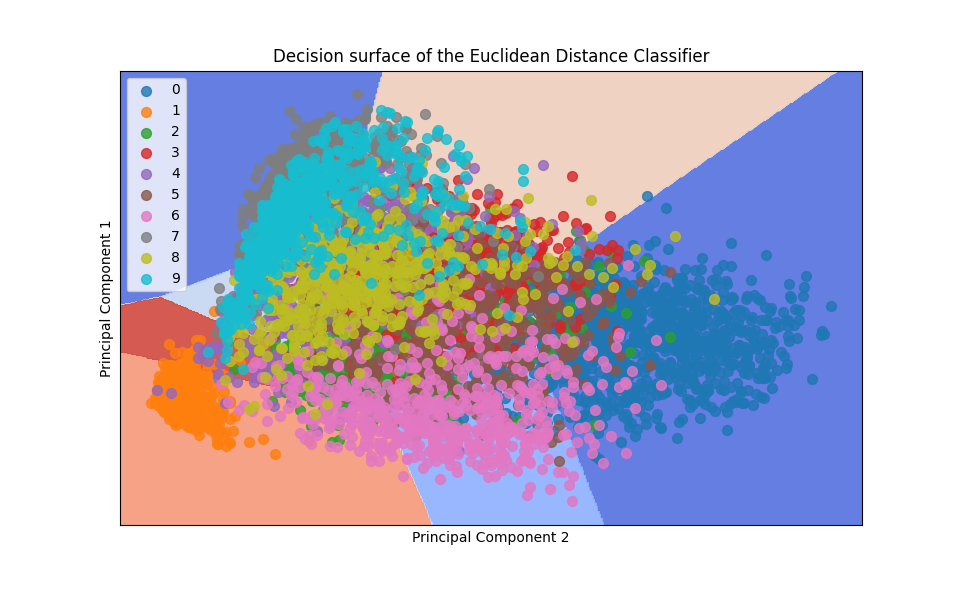
\includegraphics[width=1\textwidth]{plots/dec_surf.png}
    \caption{Η επιφάνεια απόφασης του Ευκλείδιου ταξινομητή}
    \label{fig:surface}
\end{figure}

Παρατηρούμε ότι η περιοχή απόφασης είναι αρκετά περίπλοκη, καθώς έχουμε 10 διαφορετικές κλάσεις, ανάμεσα στα διάφορα στοιχεία των οποίων υπάρχουν αρκετές αλληλοεπικαλύψεις (τουλάχιστον μετά την προβολή τους στον διδιάστατο χώρο). Για τον λόγο αυτόν ίσως είναι δύσκολο για τον Ευκλείδιο ταξινομητή να μπορέσει να πιάσει ακρίβεια μεγαλύτερη από 85\% ή 90 \%. Αν θέλουμε να πετύχουμε κάτι τέτοιο ενδεχομένως να χρειασούμε πολύ περισσότερα δεδομένα  εκπαίδευσης ή να χρησιμοποιήσουμε κάποιον άλλο ταξινομητή.\\


Τέλος σχεδιάζουμε την καμπύλη εκμάθησης του ταξινομητή μας. Αυτό γίνεται μέσω της συνάρτησης $plot\_learning\_curve$. Παίρνει ως είσοδο τον ταξινομητή (την κλάση που τον αντιπροσωπεύει) και όλα τα train δεδομένα (features, labels). 

\begin{figure}[H]
    \centering
    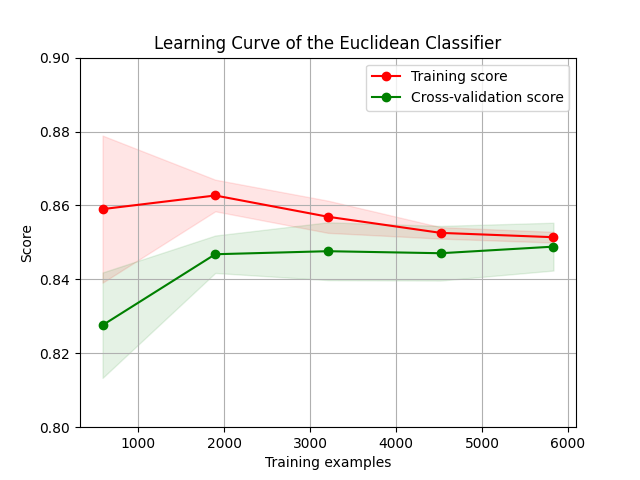
\includegraphics[width=1\textwidth]{plots/lc_eu.png}
    \caption{Η καμπύλη εκμάθησης του Ευκλείδιου ταξινομητή}
    \label{fig:learningcurve}
\end{figure}

Παρατηρούμε ότι ο ταξινομητής ξενικά από την αρχή με ψηλό cross-validation-score, το οποίο αυξάνεται αργά, μέχρι να φτάσει την οριακή του τιμή, που ταυτίζεται με το training score. Φαίνεται δηλαδή ότι η απόδοση του ταξινομητή όντως αυξάνεται καθώς έρχεται αντιμέτωπος με νέα δεδομένα.\\

\underline{\textbf{Βήμα 14}}\\

Στο \textbf{Βήμα 14} υπολογίζουμε όλες τις a-priori πιθανότητες για την κάθε κλάση (για το κάθε ψηφίο). Αυτό γίνεται πολύ απλά μετρώντας πόσες φορές εμφανίζεται το κάθε ψηφίο στο training labels και διαιρώντας με τον συνολικό αριθμό των labels. Η συνάρτηση $calculate\_priors$ κάνει ακριβώς αυτό. Παίρνει ώς είσοδο τα labels και επιστρέφει ένα dictionary το οποίο έχει ως keys τις κλάσεις  (τα ψηφία) και ως values τις αντίστοιχες πιθανότητες.\\

\begin{table}[H]
\centering
\begin{tabular}{ c c }
\hline\hline
Κλάση & A-priori Πιθανότητα \\
\hline
0  & 0.1637 \\
1 & 0.1378   \\
2  & 0.1000 \\
3 & 0.0902 \\
4 & 0.0894 \\
5 & 0.0762 \\
6 & 0.0910   \\
7 & 0.0884 \\
8 & 0.0743\\
9 & 0.0883\\
\hline
\end{tabular}
\caption{A-priori πιθανότητες για κάθε κλάση}
\label{table:a_priori}
\end{table}

Οι παραπάνω πιθανότητες δίνονται με μεγαλύτερη ακρίβεια από την κονσόλα της python (εδώ τις έχουμε στρογγυλοποιήσει). Προφανώς το άθροισμα των παραπάνω πιθανοτήτων θα πρέπει να είναι πολύ κοντά στο $1$.\\


\underline{\textbf{Βήμα 15}}\\

\textbf{(α)}: Στο \textbf{Βήμα 15} υπολοιούμε τον ταξινομητή Naive Bayes σαν έναν scikit-learn estimator, με παρόμοιο τρόπο όπως στο βήμα 12. Στην περίπτωση αυτή η κλάση που θα κατασκευάζει τον ταξινομητή είναι η CustomNBClassifier. Στην μέθοδο αρχικοποίησης εισάγουμε τέσσερεις ποσότητες:\\
1) Την λίστα με τις μέσες τιμές για την κάθε κλάση, όπως υπολογίστηκε στο βήμα 9α\\
2) Την λίστα με τις διασπορές για την κάθε κλάση, όπως υπολογίστηκε στο βήμα 9α\\
3) Τις a-priori πιθανότητες για όλες τις κλάσεις, όπως υπολογίστηκαν στο βήμα 14\\
4)Μία boolean μεταβλητή, την $use\_unit\_variance$, η οποία αρχικοποιείται ως False. Η μεταβλητή αυτή θα χρησιμοποιηθεί και σε αυτό και στο επόμενο ερώτημα για να καθορίσουμε πώς θα μοιάζει ο πίνακας συνδιακυμάνσεων που απαιτείται για τους υπολογισμούς των πιθανοτήτων στο Naive Bayes ταξινομητή.\\

Αρχικά η κλάση περιλαμβάνει την μέθοδο fit. Η μέθοδος αυτή είναι πολύ απλή και ουσιαστικά υπολογίζει τις ποσότητες που αρχικοποιήσαμε με την χρήση των train δεδομένων. Υπάρχουν όμως δύο περιπτώσεις. Αν θέσουμε αρχικά την μεταβλητή $use\_unit\_variance$ ίση με True, τότε ο πίνακας συνδιακυμάνσεων θα σχηματισθεί ως ένας $256x256$ μοναδιαίος πίνακας (κοινός για όλες τις κλάσεις). Αν είναι False, τότε ο πίνακας συνδιακυμάνσεων για μία κλάση είναι ο $256x256$ διαγώνιος πίνακας τα στοιχεία του οποίου είναι τα στοιχεία του πίνακα διασποράς της αντίστοιχης κλάσης (όπως υπολογίσθηκαν στο βήμα 9). \\

Στην συνέχεια κατασκευάζουμε μία επιπλέον μέθοδο, την $gaussian\_prob$. Η μέθοδος αυτή υπολογίζει την ποσότητα $\ln{(\mathbb{P}(X|\omega_{i})}$, δηλαδή τον λογάριθμο της δεσμευμένης πιθανότητας ενός training example δεδομένης της κλάσης. Η ποσότητα αυτή (δεδομένου ότι θεωρούμε ότι το μοντέλο μας περιγράφεται από την πολυδιάστατη κανονική κατανομή) είναι ίση με:\\
\begin{center}
$\displaystyle -\frac{256}{2} \ln{(2 \pi |Σ_{\omega_{i}}|)} - \frac{1}{2} (X - \mu_{\omega_{i}})^{T} \cdot Σ_{\omega_{i}} ^ {-1} \cdot (X - \mu_{\omega_{i}})$
\end{center}

όπου $Σ_{\omega_{i}}$ ο πίνακας συνδιακυμάνσεων της κλάσης $\omega_{i}$, $|Σ|_{\omega_{i}}$, η ορίζουσά του, $Σ_{\omega_{i}}^{-1}$ ο αντίστροφός του  και $\mu_{\omega_{i}}$ το διάνυσμα της μέσης τιμής για δεδομένη κλάση. Στην πραγματικότητα όμως, στα πλαίσια της υλοποίησης του κώδικα, προσθέσαμε κάτι παραπάνω. Επειδή τα στοιχεία του πίνακα Σ είναι μικρά (κοντά στο 0) και ο ίδιος ο πίνακας είναι διαγώνιος, η ορίζουσά του υπολογίζεται και αυτή πολύ κοντά στο 0. Αυτό προφανώς δημιουργεί πρόβλημα στον παραπάνω λογάριθμο. Για τον λόγο αυτό προσθέτουμε μέσα στον λογάριθμο έναν μικρό θόρυβο της τάξεως του $10 ^ {-6}$ και άρα ο παραπάνω τύπος γίνεται:
 \begin{center}
$\ln{(\mathbb{P}(X|\omega_{i})} = \displaystyle -\frac{256}{2} \ln{(2 \pi |Σ_{\omega_{i}}| + \epsilon)} - \frac{1}{2} (X - \mu_{\omega_{i}})^{T} \cdotΣ_{\omega_{i}}^{-1} \cdot (X - \mu_{\omega_{i}})$
\end{center}

Ένα άλλο λεπτό σημείο είναι ο υπολογισμός του αντίστροφου πίνακα $Σ ^ {-1}$. Επιλέγουμε να τον υπολογίσουμε "χειροκίνητα" καθώς είναι πολύ πιθανό βιβλιοθήκες όπως η numpy να μην είναι σε θέση να υπολογίσουν τον αντίστροφο σε περιπτώσεις όπως η δική μας. Η βιβλιοθήκη προκειμένου να ελέγξει αν ο πίνακας είναι αντιστρέψιμος, θα υπολογίσει πρώτα την ορίζουσά του και, επειδή εδώ ο πίνακας είναι διαγώνιος, η ορίζουσα θα είναι ίση με το γινόμενο των διαγώνιων στοιχείων του. Συνεπώς θα υπολογίσει μία ορίζουσα που είναι πάρα πολύ κοντά στο 0 και δεν θα συνεχίσει στον υπολογισμό του αντίστροφου. Για τον λόγο αυτό υπολογίζουμε τον αντίστροφο ως εξής: Επειδή κάποια διαγώνια στοιχεία του Σ ενδέχεται να είναι 0 (ή πολύ κοντά σε 0), προσθέτουμε σε κάθε ένα από αυτά έναν πολύ μικρό θόρυβο, ίσο με $10 ^ {-9}$. Στην συνέχεια αντικαθιστούμε κάθε διαγώνιο στοιχείο του πίνακα Σ με το αντίστροφό του (δηλαδή θέτουμε $Σ_{ii}  = \frac{1}{Σ_{ii}}$, εφόσον ο πίνακας είναι διαγώνιος). Ο θόρυβος που προσθέσαμε θα αποτρέψει σφάλματα διαιρέσεως με το 0. \\

Μετά από αυτές τις παρατηρήσεις η συνάρτηση $gaussian\_prob$ επιστρέφει τον παραπάνω λογάριθμο, που χρησιμοποιείται παρακάτω.\\


Στην συνέχεια έχουμε την μέθοδο predict, η οποία παίρνει τα test features και επιστρέφει μία λίστα με τις προβλέψεις του ταξινομητή. Αυτή λειτουργεί ως εξής: Για κάθε test example και για κάθε κλάση ψηφίων (η κάθε μία από τις οποίες χαρακτηρίζεται από μία a-priori πιθανότητα) υπολογίζει τις ποσότητες\\
\begin{center}
$\ln{\mathbb{P}(\omega_{i}|X))} = \frac{\ln{(\mathbb{P}(X|\omega_{i})) + \ln{\mathbb{P}(\omega_{i})}}}{\mathbb{P}(X)}, \hspace{0.2cm} i = 0, \dots , 9$
\end{center}

O Naive Bayes ταξινομητής μας λέει να υπολογίσουμε το $\displaystyle \operatorname*{argmax}_{i} \ln{\mathbb{P}(\omega_{i}|X)}$, που φυσικά ισούται με  $\displaystyle \operatorname*{argmax}_{i} (\ln{(\mathbb{P}(X|\omega_{i})) + \ln{\mathbb{P}(\omega_{i})}}) $. Αυτό γίνεται αρχικοποιώντας μία άδεια λίστα για το κάθε test example, μέσα στην οποία θα προσθέσουμε όλες τις παραπάνω πιθανότητες. Όταν Η λίστα αυτή (για δεδομένο Χ) έχει 10 αριθμούς, δηλαδή και τους 10 παραπάνω λογαρίθμους, θα επιλέξουμε το index της λίστας που περιέχει τον μεγαλύτερο αριθμό (θεωρούμε ότι οι πιθανότητες υπολογίζονται και προσθέτονται στην λίστα με την σειρά των ψηφίων, δηλαδή πρώτα η $\ln{\mathbb{P}(\omega_{0}|X))}$, μετά η $\ln{\mathbb{P}(\omega_{1}|X))}$ κ.ο.κ.). Παίρνουμε έτσι ένα index, το οποίο ταυτίζεται με την κλάση του ψηφίου στην οποία ταξινομήθηκε το εν λόγω example. Αυτή η πρόβλεψη μπαίνει με την σειρά της σε μία άλλη λίστα. Όταν η παραπάνω διαδικασία γίνει για όλα τα test examples, επιστρέφουμε την λίστα με τις προβλέψεις.\\

Τέλος έχουμε την μέθοδο score. Αυτή υπολογίζει την λίστα με τις προβλέψεις μέσω της predict, υπολογίζει πόσα στοιχεία από την λίστα αυτή είναι ίσα με τα test labels και διαιρεί με το μήκος της λίστας των test labels.\\

\textbf{(β)}: Για να υπολογίσουμε το score, αρχικά κατασκευάζουμε τον ταξινομητή και καλούμε με την σειρά τις μεθόδους fit και score 

\begin{center}
clf = CustomNBClassifier(use unit variance = False)\\
clf.predict(our test features)\\
clf.score(our test features, our test labels)\\
\end{center}

Η μεταβλητή $use\_unit\_variance$ τίθεται ίση με False και άρα θα χρησιμοποιήσουμε σαν πίνακα συνδιασπορών τις διασπορές του βήματος 9. Αν το κάνουμε αυτό θα πάρουμε ένα score ίσο με 82.2\%. Φαίνεται δηλαδή ότι παίρνουμε παραπλήσιο score με αυτό του Ευκλείδιου ταξινομητή. Αυτό ενδεχομένως να οφείλεται στις υπερβολικά απλοϊκές παραδοχές που έχουμε κάνει προκειμένου να υλοποιήσουμε τον ταξινομητή Naive Bayes ή στους θορύβους που έχουμε επιλέξει να προσθέσουμε για τους διάφορους υπολογισμούς.\\

\textbf{(γ)}: Ο ταξινομητής του sklearn που αντιστοιχεί στον Naive Bayes είναι ο GaussianNB. Αν τον καλέσουμε με αντίστοιχες εντολές, όπως του βήματος 15β, τότε θα υπολογίσουμε ένα score ίσο με 71.94\%. Αυτό το αποτέλεσμα είναι τουλάχιστον εκπληκτικό καθώς το score αυτό βγαίνει μικρότερο απο εκείνο του ταξινομητή που υλοποιήσαμε στα προηγούμενα ερωτήματα. Αυτό πρέπει να οφείλεται καθαρά στο πώς το sklearn υλοποιεί τον ταξινομητή αυτόν και όχι σε κάποιο ενδογενές χαρακτηριστικό των δεδομένων. Ένα πιθανό ενδεχόμενο είναι στο sklearn να χρησιμοποιούνται διαφορετικοί θόρυβοι ($var\_smoothing$) για τον υπολογισμό οριζουσών και πινάκων (δηλαδή να λειτουργούν ως υπερπαράμετροι του μοντέλου) ή να υπολογίζονται με διαφορετικό τρόπο οι πίνακες συνδιακυμάνσεων των κλάσεων (έτσι ώστε τα δεδομένα να καθίστανται ανεξάρτητα κατανεμημένα). \\

Παρόλα αυτά θα περίμενε κανείς ότι όντως το score του Naive Bayes ταξινομητή θα βγαίνει μικρότερο από αυτό του Ευκλείδιου ταξινομητή, καθώς τα δεδομένα μας δεν είναι στην πραγματικότητα πλήρως ανεξάρτητα κατανεμημένα. \\

\underline{\textbf{Βήμα 16}}\\

Στο \textbf{Βήμα 16} χρησιμοποιούμε την ίδια ακριβώς κλάση με το βήμα 15, μόνο αυτή την φορά, όταν κατασκευάζουμε τον ταξινομητή, φροντίζουμε να θέσουμε την boolean μεταβλητή $use\_unit\_variance = True$. Αυτό θα έχει ως αποτέλεσμα ο πίνακας των συνδιακυμάνσεων να είναι ο μοναδιαίος πίνακας διαστάσεων $256x256$. Για να υπολογίσουμε το score κάνουμε ακριβώς τα ίδια βήματα με το βήμα 15, δηλαδή πρώτα κάνουμε fit τα train δεδομένα και στην συνέχεια καλούμε την μέθοδο score στα test δεδομένα. Αν το κάνουμε αυτό θα πάρουμε ένα score ίσο με 81.26\%.\\

Το score αυτό είναι λογικό και αναμενόμενο και είναι (προσεγγιστικά) ίσο με το score του Ευκλείδιου ταξινομητή του βήματος 12. Ο Ευκλείδιος ταξινομητής είναι στην ουσία μία ειδική περίπτωση του Naive Bayes ταξινομητή, όταν ισχύουν οι εξής προϋποθέσεις:\\
1) Όλα τα train δεδομένα ακολουθούν την ίδια κατανομή και είναι κατανεμημένα με τον ίδιο τρόπο (Independent and identically distributed)\\
2) Το μοντέλο (δηλαδή οι δεσμευμένες πιθανότητες $\mathbb{P}(X|\omega_{i})$) περιγράφεται από την κανονική κατανομή\\
3) Ο πίνακας συνδιακυμάνσεων είναι μοναδιαίος\\

Οι προϋποθέσεις (1) και (2) ισχύουν στο βήμα 15. Στο βήμα 16 ουσιατικά προστέθηκε η τρίτη παραδοχή που καθιστά τον Naive Bayes ταξινομητή ισοδύναμο με τον Ευκλείδιο ταξινομητή. Για τον λόγο αυτό παίρνουμε και το ίδιο score.\\

\underline{\textbf{Βήμα 17}}\\

Στο \textbf{Βήμα 17} συγκρίνουμε την απόδοση (το score) διάφορων ταξινομητών της βιβλιοθήκης Scikit-learn. Οι ταξινομητές που θα συγκρίνουμε θα είναι οι GaussianNB (ο γνωστός και από το βήμα 15 Naive Bayes ταξινομητής), KNeighborsClassifier (ταξινόμηση με βάση τους κοντινότερους $Κ$ (στην περίπτωσή μας 5) γείτονες του κάθε στοιχείου) και SVM (Support Vector Machines) με γραμμικό και radial-basis-function πυρήνες. Δανειζόμαστε κατά τα γνωστά τις αντίστοιχες κλάσεις από το Scikit-learn, κάνουμε fit τα train δεδομένα και στην συνέχεια παίρνουμε τις προβλέψεις μας μέσω της μεθόδου predict για τα test δεδομένα. Αυτό γίνεται με την συνάρτηση $compare\_classifiers$ που παίρνει ως είσοδο τα train δεδομένα. Αν την καλέσουμε, θα δούμε στην οθόνη μας:\\
\begin{center}
Sklearn Gaussian Naive Bayes estimator gives a score of: 71.95 \%\\
Sklearn K-Neighbors estimator gives a score of: 94.47 \%\\
Sklearn SVM with linear kernel estimator gives a score of: 92.63 \%\\
Sklearn SVM with rbf kernel estimator gives a score of: 94.72 \%\\
\end{center}

Το πρώτο πράγμα που παρατηρούμε είναι ότι ο ταξινομητής που βγαίνει αμέσως εκτός ανταγωνισμού είναι ο Naive Bayes ταξινομητής. Φαίνεται ότι τα δεδομένα μας κρύβουν μεγάλη αβεβαιότητα και η ταξινόμησή τους με βάση πιθανοκρατικές μεθόδους είναι πολύ δύσκολη. Η παραδοχή ότι ο πίνακας συνδιασποράς είναι διαγώνιος και αποτελείται από τις διασπορές του εκάστοτε pixel της κλάσης ενός ψηφίου ενδεχομένως να εμποδίζει τον ταξινομητή να εντοπίσει κρυμμένα μοτίβα μέσα στα δεδομένα.\\

Οι επόμενοι τρεις ταξινομητές φαίνεται να πετυχαίνουν παρόμοια απόδοση, με κορυφαίο ταξινομητή τα Support Vector Machines με RBF-πυρήνα. Ο αλγόριθμος των SVM  προσπαθεί να βρει ένα υπερεπίπεδο που να διαχωρίζει "όσο το δυνατόν καταλληλότερα" (με βάση κάποιο κριτήριο βελτιστοποίησης) τα δεδομένα μας. Για να επιτευχθεί αυτό πολλές φορές τα δεδομένα επεκτείνονται σε έναν χώρο ακόμα μεγαλύτερης διάστασης από αυτόν που ζουν προκειμένου να είναι διαχωρίσιμα (όπως π.χ. στο πρόβλημα XOR). Στην συνέχεια ο πυρήνας ορίζει το "σχήμα" της υπερεπιφάνειας που θα διαχωρίσει τα δεδομένα. Προφανώς ένας μη-γραμμικός πυήνας θα είναι εν γένει πιο ικανός να "ελίσσεται" στον υπερχώρο του προβήματος και να προσφέρει μία ενδεχομένως καμπυλομένη επιφάνεια που θα λάβει υπόψην όλες τις παραπάνω πληροφορίες που αποκτούν τα δεδομένα από την αύξηση της διαστατικότητάς τους.\\

Ο ταξινομητής Κ-Neighbors δίνει επίσης ένα πολύ ικανοποιητικό score. Αυτό ενδεχομένως να σημαίνει ότι τα train δεδομένα μας, τα οποία ζουν σε ένα χώρο 256 διαστάσεων, είναι συσταδισμένα (clustered) σε ικανοποιητικό βαθμό που τα test δεδομένα να μπορούν να ταξινομούνται με πολύ μικρή αβεβαιότητα στις διαφορετικές συστάδες (clusters).\\

Τέλος, για χάρη παραπάνω οπτικοποίησης, δίνουμε και τα Confusion Matrices των ταξινομητών αυτών:\\

\begin{figure}[H]
    \centering
    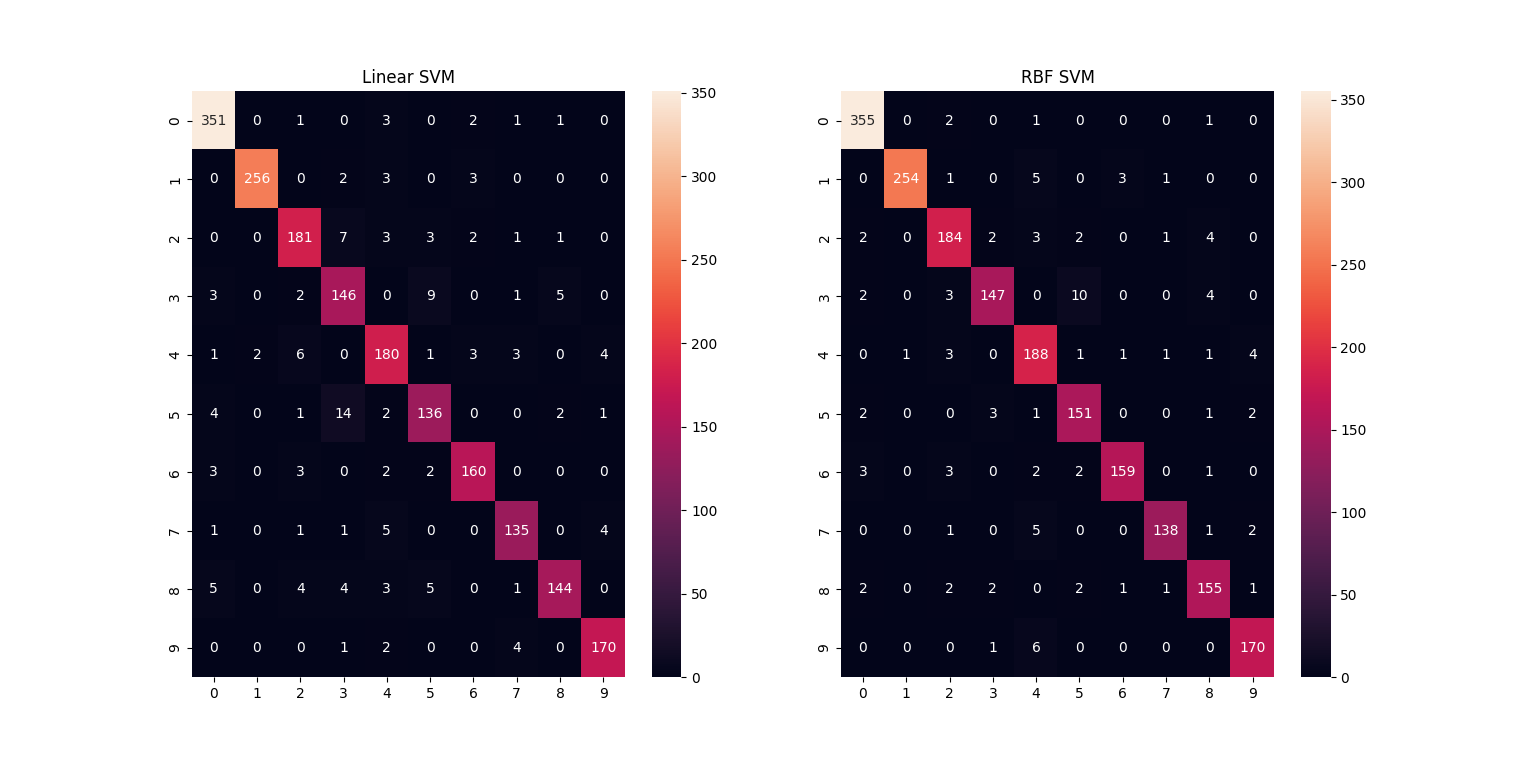
\includegraphics[width=1.2\textwidth]{plots/cm_svms.png}
    \caption{Τα Confusion Matrices των SVM}
    \label{fig:cm_svm}
\end{figure}

\begin{figure}[H]
    \centering
    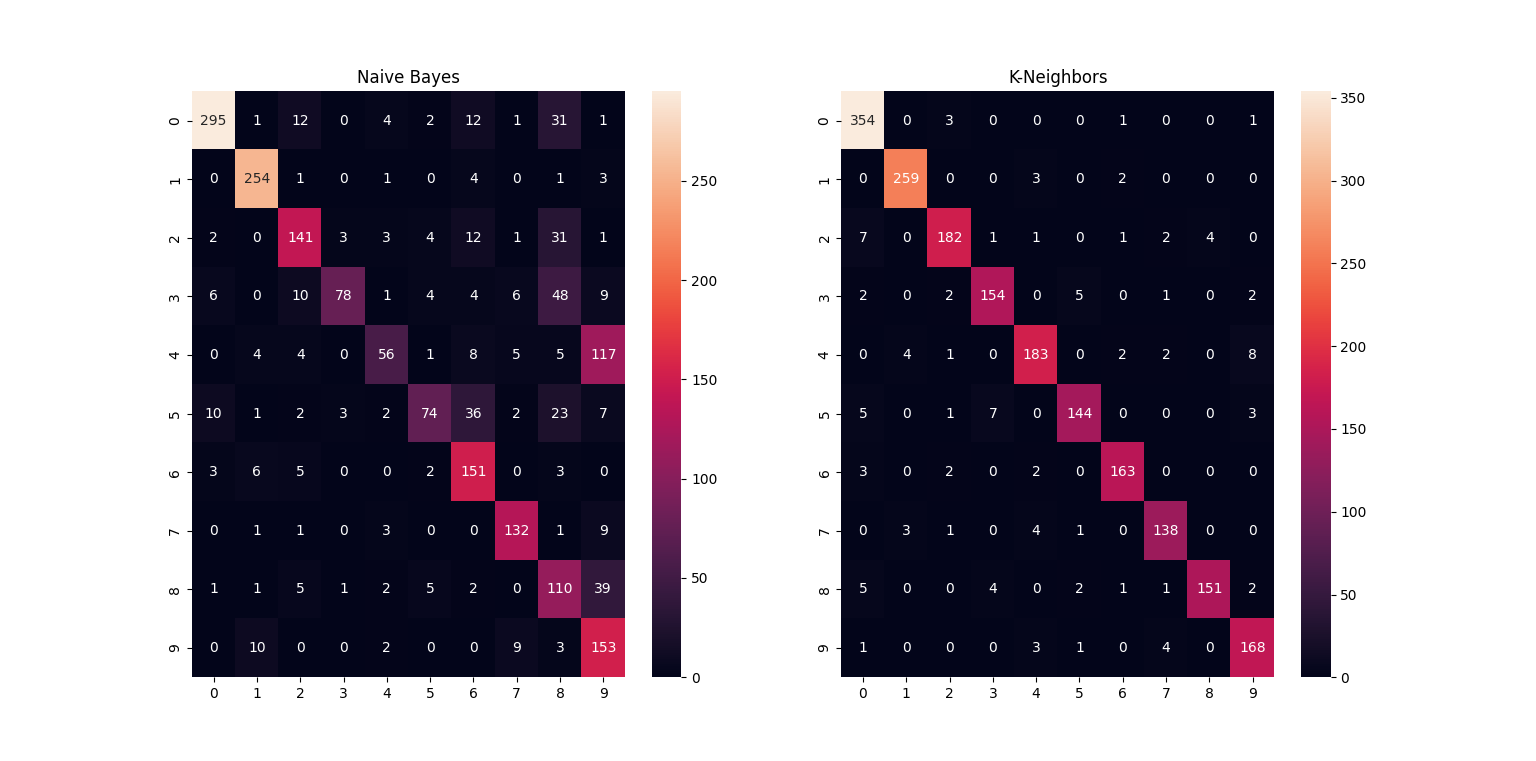
\includegraphics[width=1.2\textwidth]{plots/cm_k_n.png}
    \caption{Τα Confusion Matrices των Naive Bayes και K-Neighbors}
    \label{fig:cm_kn}
\end{figure}

Η ακρίβεια του ταξινομητή μπορεί να υπολογισθεί από τo Confusion Matrix του διαιρώντας το ίχνος του με το άθροισμα όλων των στοιχείων του. Πέρα από αυτό όμως μπορεί να μας δείξει επιπλεόν πληροφορίες που σχετίζονται με το σφάλμα του ταξινομητή. Γενικά θέλουμε τα στοιχεία της διαγωνίου να είναι μεγάλα και όλα τα υπόλοιπα μικρά. Ας δούμε που δεν συμβαίνει αυτό στο Confusion Matrix του Naive Bayes. Αν δούμε την γραμμή με index 4 και την στήλη με index 9, ο αριθμός είναι ίσος με 117. Αυτό σημαίνει ότι ο ταξινομητής 117 στοιχεία που είχαν label 4 τα κατέταξε (προέβλεψε) στην κλάση με label 9. Αντίστοιχα συμπεράσματα βγαίνουν και για τα υπόλοιπα μη-διαγώνια στοιχεία, μερικά από τα οποία είναι μεγάλα. Για τους υπόλοιπους τρεις ταξινομητές τα μη-διαγώνια στοιχεία είναι πολύ μικρά και γι'αυτό το score τους είναι μεγάλο.\\

\underline{\textbf{Βήμα 18}}\\

Στο βήμα αυτό εξετάζονται δύο διαφορετικές μέθοδοι συνδυασμού πολλαπλών ταξινομητών για την ταξινόμηση των δειγμάτων, οι οποίες ανήκουν στη γενικότερη κατηγορία μεθόδων ensembling. Στο πρώτο στάδιο εξετάζεται η μέθοδος του Voting Classifier (από τη βιβλιοθήκη του scikit-learn). Η συγκεκριμένη μέθοδος επιστρατεύει τη χρήση πολλαπλών ταξινομητών για την ταξινόμηση των δειγμάτων, χρησιμοποιώντας τους παράλληλα και στο τέλος απόφασίζει σε ποια κλάση θα ταξινομηθεί ένα δείγμα με βάση μια διαδικασία που ονομάζεται voting. Η διαδικασία του voting διακρίνεται σε hard και soft. Στην πρώτη περίπτωση, η τελική απόφαση του ταξινομητή συμπίπτει με την απόφαση της πλειοψηφίας των ταξινομητών, δηλαδή αν σε ένα υποθετικό παράδειγμα οι τρεις ταξινομητές που χρησιμοποιούνται ταξινομούν ένα δείγμα στις κλάσεις (Α,Α,Β) αντίστοιχα, τότε η τελική απόφαση θα είναι να ταξινομηθεί στην κλάση Α. Στην περίπτωση του soft voting, το αποτέλεσμα προκύπτει με βάση τις πιθανότητες που δίνει ο κάθε ταξινομητής για να ταξινομηθεί ένα δείγμα στην κάθε κλάση και σαν τελική απόφαση επιλέγεται η κλάση με τη μεγαλύτερη πιθανότητα. Επιπλέον, στην περίπτωση του hard voting συστήνεται η χρήση περιττού αριθμού ταξινομητών έτσι ώστε να αποφεύγονται καταστάσεις "ισοπαλίας", δηλαδή η περίπτωση στην οποία οι δυο πρώτοι ταξινομητές επιλέγουν την κλάση Α και οι δύο άλλη επιλέγουν την κλάση Β για το ίδιο δείγμα. \\

Για τους σκοπούς της άσκησης χρησιμοποιήθηκαν τρεις ταξινομητές για τη διαδικασία του hard voting: ο ταξινομητής Gaussian Naive Bayes, ο K-Neighbors και ο SVM (linear kernel) από τη βιβλιοθήκη του scikit-learn, ακολουθώντας τον κανόνα για περιττό αριθμό ταξινομητών. Η επιλογή αυτών των ταξινομητών βασίστηκε στη λογική συνδυασμού ενός ταξινομητή με αισθητά χαμηλότερη ακρίβεια (Gaussian Naive Bayes) με δύο άλλους ταξινομητές που που έχουν μεγαλύτερη ακρίβεια. Αυτή η σκέψη είναι συμβατή με τη γενικότερη φιλοσοφία του voting classifier, η οποία προτείνει το συνδυασμό ταξινομητών οι οποίοι αποτυγχάνουν σε διαφορετικές περιπτώσεις δειγμάτων ο ένας από τον άλλον.\\

Στο δεύτερο στάδιο, εξετάστηκε η εφαρμογή της ensembling μεθόδου Bagging Classifier. Η περίπτωση αυτή διαφέρει σε σχέση με τον απλό voting classifier που περιγράφθηκε προηγουμένως, καθώς το bagging (bootsrap aggregation) αναφέρεται στο διαχωρισμό των training δεδομένων σε $n$ στο πλήθος μικρότερα datasets, τα οποία εμφανίζουν και επικαλύψεις. Στη συνέχεια, επιλέγεται ένας ταξινοητής ο οποίος θα εκπαιδευταί $n$ φορές εξ αρχής, κάθε φορά σε ένα διαφορετικό dataset. Μέσω αυτής της διαδικασίας θα έχουν προκύψει $n$ διαφορετικοί ταξινομητές, οι οποίοι στη συνέχει θα κληθούν να ταξινομήσουν σε κλάσεις όλα τα δεδομένα του αρχικού dataset. Η τελική απόφαση για την ταξινόμηση ενός δείγματος γίνεται με βάση με μία αντίστοιχη διαδικασία voting, όμοια με αυτή που αναλύθηκε προηγουμένως. Ο κύριος σκοπός της μεθοδολογίας του bagging classification επικεντρώνεται στην αναγνώριση ταξινομητών οι οποίοι μπορεί να είναι ασταθείς (unstable), δηλαδή ταξινομητών οι οποίοι εμφανίζουν σημαντικά διαφορετική (προβλεπτική) συμπεριφορά όταν εκπαιδεύονται με ελαφρώς διαφορετικά training δεδομένα. Έτσι, εκπαιδεύοντας έναν τύπο (ασταθούς) ταξινομητή πολλαπλές φορές σε ελαφρώς διαφορετικά training δεδομένα, οδηγούμαστε σε μείωση της διακύμανσης τως προβλέψεων.\\

Για τον έλεγχο αυτής της μεθόδου χρησιμοποιήθηκε ξανά ο Gaussian Naive Bayes Classifier. Τόσο στην περίπτωση του Voting Classifier όσο και στου Bagging Classifier εφαρμόστηκε 5-fold Cross Validation ώστε να ελεγχθεί η βελτίωση της ακρίβειας των ταξινομητών ensembling. Τα αναλυτικά αποτελέσματα της ακρίβειας των δύο μεθόδων παρουσιάζονται αναλυτικά στον πίνακα \ref{tab:ansemble-accuracies}.\\

Παρατηρώντας τα αποτελέσματα του πίνακα \ref{tab:ansemble-accuracies} προκύπτει ότι η μέθοδος του voting classifier, δηλαδή ο συνδυασμός των τριών διαφοεριτικών ταξινομητών οδήγησε σε υψηλά ποσοστά ακρίβειας. Το αποτέλεσμα αυτό θα μπορούσε να θεωρηθεί αναμενόμενο, καθώς οι δύο από τους τρείς ταξινομητές που χρησιμοποιήθηκαν είχαν από μόνοι τους πολύ υψηλά ποσοστά ακρίβειας (της τάξης του 90 \%), επομένως, οι προβλέψεις τους συμφωνούν και διορθώνουν τις προβλέψεις του Gaussian Naibe Bayes ταξινομητή. Επιπλέον, η εφαρμογή του 5-fold Cross Validation βελτίωση ελαφρώς τις επιδόσεις και των δυο ταξινομητών, όπως ήταν αναμενόμενο. Τέλος, φαίνεται πως ο Bagging Classiafier δεν επιφέρει βελτίωση του ποσοστού ακρίβειας του Naive Bayes ταξινομητή, κάτι το οποίο ήταν αναμενόμενο για τη συγκεκριμένη μεθοδολογία ensembling. \\

\begin{table}[h]
\begin{center}
\begin{tabular}{c c }
\hline\hline
Μοντέλο & Ακρίβεια\\
\hline
Voting Classifier & 93.52 \%\\ 
Voting Classifier (5-fold Cross-val.) & 95.39 $\pm$  0.53 \%\\  
Bagging Classifier & 71.60 \%\\
Voting Classifier (5-fold Cross-val.) & 74.28 $\pm$ 2.26 \%\\
\hline 
\end{tabular}
\caption{Ποσοστά ακρίβειας των μεθόδων ensembling που δοκιμάστηκαν.}
\label{tab:ansemble-accuracies}
\end{center}
\end{table}

\underline{\textbf{Βήμα 19}}\\

Στο τελευταίο αυτό βήμα (\textbf{Βήμα 19}) κατασκευάζουμε ένα νευρωνικό δίκτυο με την χρήση του Pytorch το οποίο θα λειτουργήσει ως ταξινομητής. Η κλάση που θα περιλαμβάνει το δίκτυο και τις λειτουργίες του είναι η PytorchNNModel, ενώ η συνάρτηση που θα την επικαλείται για να μας δώσει τις προβλέψεις και τα scores είναι η $evaluate\_nn\_classifier$. Η συνάρτηση αυτή κάνει fit τα train δεδομένα και στην συνέχεια υπολογίζει το accuracy και το cross-validation-score.\\

 Για όλες τις δοκιμές που θα ακολουθήσουν αναφέρουμε πρώτα τις παραμέτρους που θα παραμείνουν σταθερές σε όλες τις δοκιμές:

\begin{itemize}
\item \textbf{Συνάρτηση Κόστους}: Επειδή το πρόβλημά μας είναι πρόβλημα ταξινόμησης σε διακριτές κλάσεις, η καταλληλότερη συνάρτηση κόστους που μπορεί κανείς να επιλέξει είναι η \textit{CrossEntropyLoss}.\\
\item \textbf{Optimizer}: Είναι ο αλγόριθμος που θα ανανεώνει σε κάθε επανάληψη τα βάρη του νευρωνικού δικτύου. Επιλέγεται ο \textit{Adam Optimizer}\\
\item \textbf{Batch Size}: Επειδή το πρόβλημα που έχουμε είναι αρκετά απλό και τα δεδομένα μικρά σε όγκο, επιλέξαμε να τροφοδοτήσουμε όλα τα δεδομένα μαζι στο δίκτυο σε κάθε επανάληψη. Σε περίπτωση που τα δεδομένα μας είναι πολύ μεγαλύτερα σε όγκο, τότε θα πρέπει (και για λόγους μνήμης και χρόνου) να χωρίσουμε τα δεδομένα μας σε batches. Παρόλα αυτά δεν αναμένουμε πολύ διαφορετικά αποτελέσματα αν χρησιμοποιήσουμε batches. Αν θέλουμε να υλοποιήσουμε τον ίδιο αλγόριθμο αλλά χωρίζοντας πρώτα τα featureds και τα labels σε batches, μπορούμε να χρησιμοποιήσουμε την κλάση $PytorchNNModel\_with\_batches$\\
\item \textbf{Αριθμός εποχών}: Επιλέγεται ίσος με 100. \\
\end{itemize}

Μέσα στην κλάση PytorchNNModel αρχικοποιούνται τα εξής: 1) Το μοντέλο του νευρωνικού δικτύου (μέσω της κλάσης Sequential), δηλαδή το πόσα κρυφά στρώματα θα έχει, πόσους νευρώνες ανά στρώμα θα έχει και τι είδους συναρτήσεις ενεργοποίησης θα περιέχει, 2) Η συνάρτηση κόστους του δικτύου και 3)Ο αλγόριθμος που θα ανανεώνει τα βάρη του δικτύου (optimizer).\\


\textbf{Δοκιμή 1η}

Σε αυτήν την προσωμοίωση η αρχιτεκτονική του δικτύου είναι η εξής: Περιλαμβάνει δύο γραμμικά κρυφά στρώματα με 200 νευρώνες το καθένα. Όλες οι συναρτήσεις ενεργοποίησης είναι ReLU.\\

Αν καλέσουμε την συνάρτηση $evaluate\_nn\_classifier$ δίνοντάς της τα train δεδομένα θα πάρουμε στην οθόνη μας:\\
\begin{center}
Neural Network estimator gives an accuracy of: 93.57 \% \\
The 5-fold cross-validation score of the Neural Network classifier is 96.95 +-0.29
\end{center}

Παρατηρούμε από το cross-validation και μόνο ότι το νευρωνικό αυτό είναι παραπάνω από ικανό να γενικεύσει την δράση του σε ένα άγνωστο set δεδομένων. Επίσης το score του νευρωνικού είναι αρκετά ικανοποιητικό, ειδικά για τόσο μικρό όγκο δεδομένων.\\

\textbf{Δοκιμή 2η}

Σε αυτήν την δοκιμή αλλάζουμε όλες τις συναρτήσεις ενεργοποίησης από ReLU σε Sigmoid. Αυτήν την φορά θα πάρουμε:\\
\begin{center}
Neural Network estimator gives an accuracy of: 92.88 \% \\
The 5-fold cross-validation score of the Neural Network classifier is 95.90 +-0.15
\end{center}

Σε αυτήν την περίπτωση τα νούμερα είναι ελαφρώς χαμηλότερα αλλά χωρίς καμία ουσιώδη διαφορά. Παρόμοια αποτελέσματα θα λάβουμε αν τρέξουμε το νευρωνικό με υπερβολικές εφαπτομένες.\\

\textbf{Δοκιμή 3η}

Σε αυτήν την δοκιμή δίνουμε στο νευρωνικό ένα μόνο γραμμικό κρυφό στρώμα με 200 νευρώνες και συναρτήσεις Sigmoid. Λαμβάνουμε:\\
\begin{center}
Neural Network estimator gives an accuracy of: 92.27 \% \\
The 5-fold cross-validation score of the Neural Network classifier is 95.70 +-0.29
\end{center}

Και εδώ παίρνουμε παρόμοια αποτελέσματα. Φαίνεται λοιπόν ότι ακόμα και ένα "απλό" νευρωνικό δίκτυο είναι ικανό να λύσει ένα τόσο απλό πρόβλημα όπως η ταξινόμηση των ψηφίων. Δεν φαίνεται η αρχιτεκτονική του να επηρεάζει ιδιαίτερα το performance του αλγορίθμου. Η μόνη κρίσιμη παράμετρος που ενδεχομένως να δείξει κάτι διαφορετικό είναι ο ρυθμός εκμάθησης του Adam, όπου για κάποιο εύρος τιμών ενδέχεται το νευρωνικό να μην συγκλίνει ή να συγκλίνει πιο αργά. Κάνουμε μία τελευταία δοκιμή. \\

\textbf{Δοκιμή 4η}

Στην δοκιμή αυτή παίρνουμε την ίδια αρχιτεκτονική με την τρίτη δοκιμή και απλώς αλλάζουμε τον ρυθμό εκμάθησης του Adam από 0.005 σε 0.001. Παίρνουμε:\\
\begin{center}
Neural Network estimator gives an accuracy of: 89.18 \% \\
The 5-fold cross-validation score of the Neural Network classifier is 92.69 +-0.32
\end{center}

Παρατηρούμε ότι η αλλαγή του ρυθμού εκμάθησης έκανε την μοναδική πραγματική διαφορά, καθώς έριξε το score κάτω από το 90 \%. Ενδεικτικά, ένας τρόπος να λύσουμε το πρόβλημα αυτό, αν θέλουμε να κρατήσουμε τον ρυθμό εκμάθησης ίσο με 0.001 θα είναι να αυξήσουμε τις εποχές του αλγορίθμου. \\

Ενδεικτικά στην τελευταία αυτή περίπτωση δίνουμε και την καμπύλη εκμάθησης του ταξινομητή:
\begin{figure}[H]
    \centering
    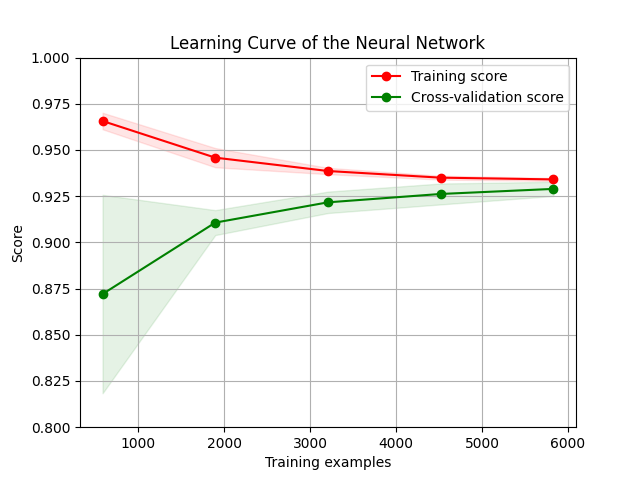
\includegraphics[width=1\textwidth]{plots/lc_nn.png}
    \caption{Η καμπύλη εκμάθησης του Νευρωνικού Δικτύου}
    \label{fig:nn_lc}
\end{figure}

Το cross-validation-score του δικτύου αυξάνεται πάρα πολύ γρήγορα ήδη από τα αρχικά στάδια της εκπάιδευσης, κάτι που δείχνει ότι ικανότητά του να αναγνωρίζει τα πρότυπα που εμφανίζονται στα δεδομένα αυξάνεται και αυτή καθώς προχωρά η εκπαίδευσή του.\\

Προγανώς οι υπερπαράμετροι είναι πάρα πολλοί και πρέπει να ελέγχεται ο καθένας ξεχωριστά, κρατώντας τους υπόλοιπους σταθερούς για να βγει κάποιο συνεπές συμπέρασμα.\\

 
\end{document}